%%%%%%%%%%%%%%%%%%%%%%%
%
%   Question 4
%
%%%%%%%%%%%%%%%%%%%%%%%

{\textsc{\underline{Question 4 sur les relations  (\textbf{20} points)}}}\\

Les parties A et B sont \underline{ind\'ependantes}.\\

\textbf{Partie A} (12 points)\\

 Soit $R$ la relation sur l'ensemble $A=\{0, 1,2,3,4,5,6,7,8 \}$ d\'efinie par 
$$xRy \Longleftrightarrow x = y - 3 \quad(\mbox{on note aussi }(x,y) \in R). $$ 

\begin{enumerate}[\bf 1.]

\item\bareme{2} Dessiner le graphe de $R$.
%%%%%%%%%%%%%%%%%%%%%%%%%%%%%%% 
% Solution                    %
%%%%%%%%%%%%%%%%%%%%%%%%%%%%%%%
\begin{framed}

R\'EPONSE:
\vspace{-.75cm}
\begin{center}
    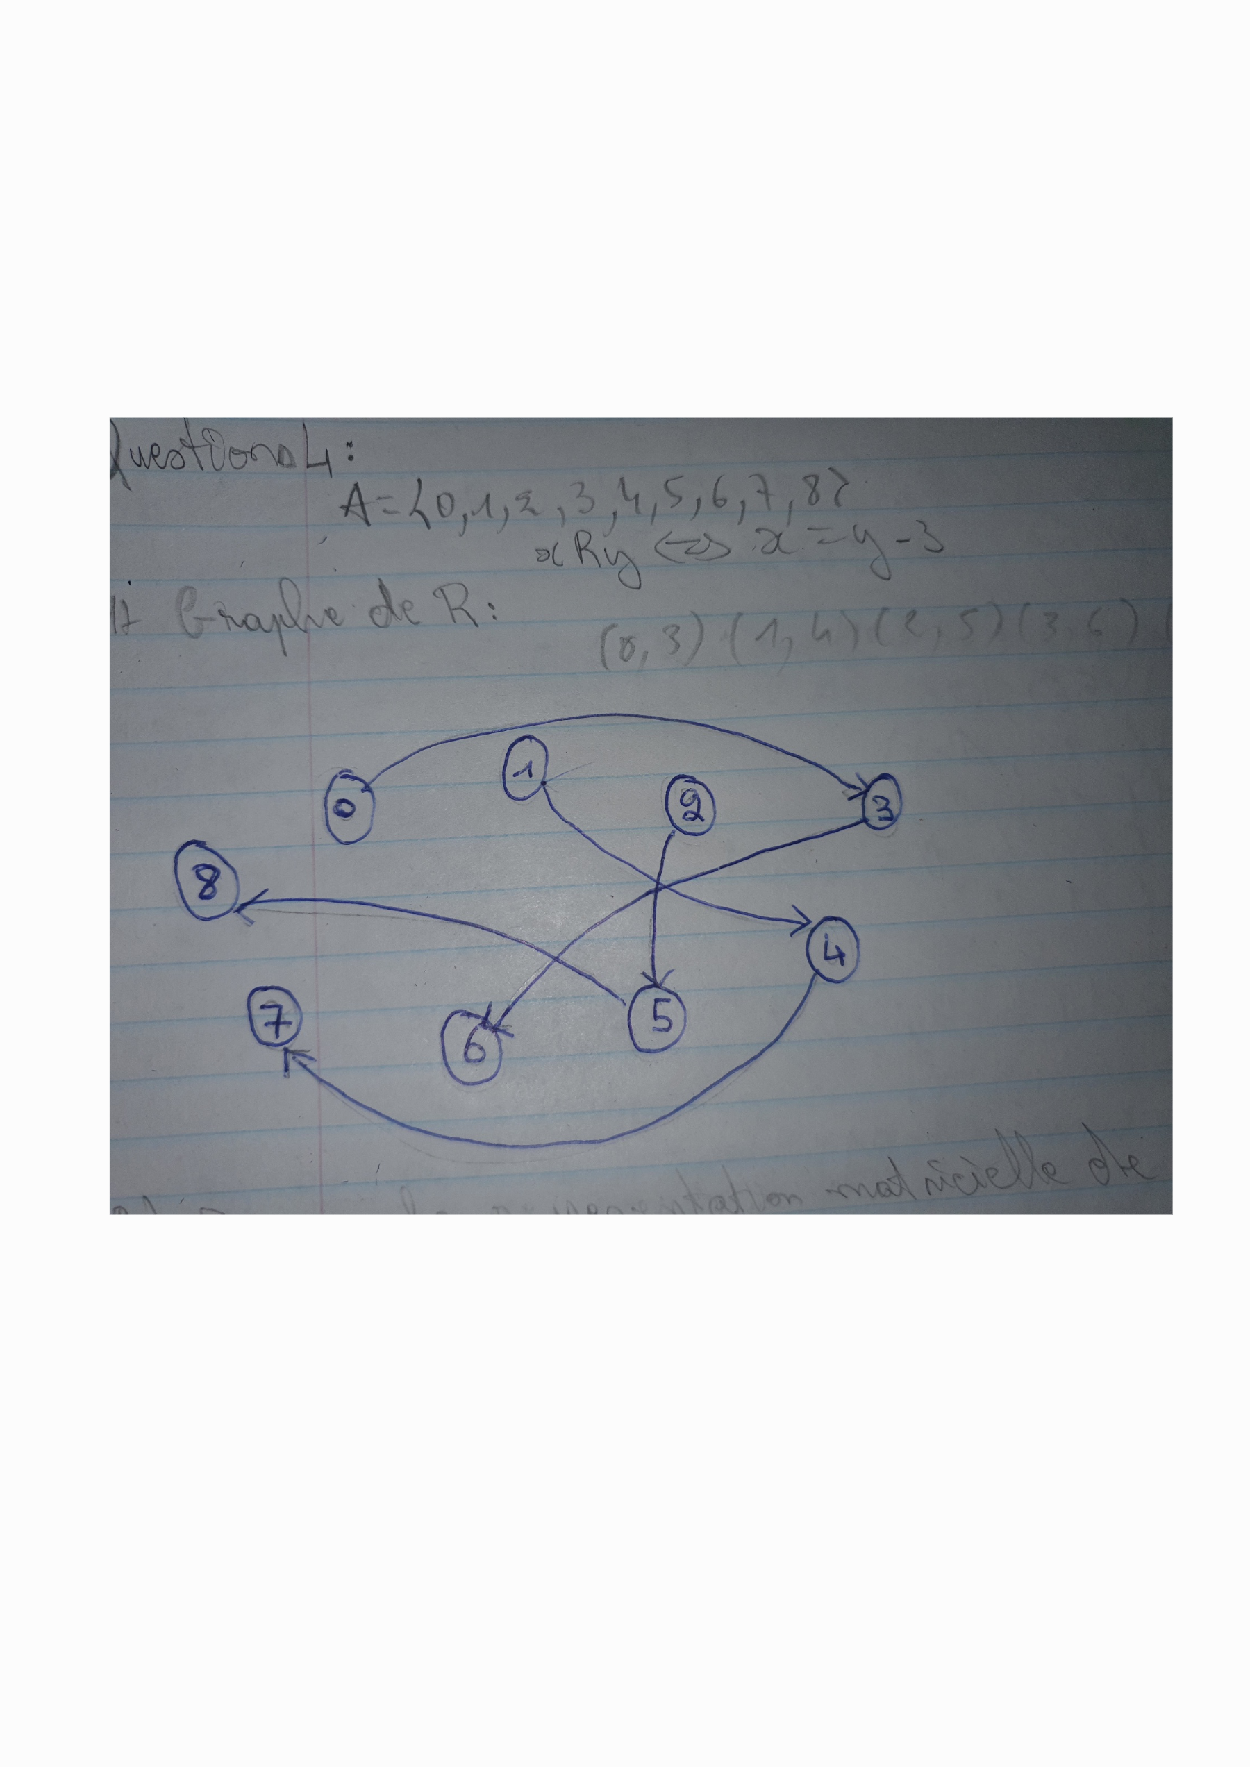
\includegraphics[width=3.5 in]{Figures/Graphe1.pdf} 
\end{center}
\vspace{-.75cm}
\end{framed}
%%%%%%%%%%%%%%%%%%%%%%%%%%%%%%%
\item\bareme{2} Donner la représentation matricielle de $R$.
%%%%%%%%%%%%%%%%%%%%%%%%%%%%%%% 
% Solution                    %
%%%%%%%%%%%%%%%%%%%%%%%%%%%%%%%
\begin{framed}

R\'EPONSE:
 $M_R$= 
 \begin{bmatrix}
 0&0 &0&1&0&0&0&0&0\\
 0&0 &0&0&1&0&0&0&0\\
 0&0 &0&0&0&1&0&0&0\\
 0&0 &0&0&0&0&1&0&0\\
 0&0 &0&0&0&0&0&1&0\\
 0&0 &0&0&0&0&0&0&1\\
 0&0 &0&0&0&0&0&0&0\\
 0&0 &0&0&0&0&0&0&0\\
 0&0 &0&0&0&0&0&0&0\\
\end{bmatrix}

\end{framed}
%%%%%%%%%%%%%%%%%%%%%%%%%%%%%%%
\item\bareme{2} La relation $R$ est-elle réflexive? symétrique? antisymétrique? Justifiez vos réponses.
%%%%%%%%%%%%%%%%%%%%%%%%%%%%%%% 
% Solution                    %
%%%%%%%%%%%%%%%%%%%%%%%%%%%%%%%
\begin{framed}

R\'EPONSE: \\
La relation $R$ n'est pas réflexive car $x$ n'est pas en relation avec lui même. \\
La relation $R$ n'est pas symétrique car $(x,y) \in R$ mais $(y,x)$ n'appatient pas à $R$ \\
La relation $R$ est  antisymétrique car $(x,y) \in R$ mais $(y,x)$ n'appatient pas à $R$ \\
\end{framed}
%%%%%%%%%%%%%%%%%%%%%%%%%%%%%%%
\item\bareme{2} Soit $T$ la fermeture transitive de $R$. Dessiner le graphe ou donner la matrice de $T$.
%%%%%%%%%%%%%%%%%%%%%%%%%%%%%%% 
% Solution                    %
%%%%%%%%%%%%%%%%%%%%%%%%%%%%%%%
\begin{framed}

R\'EPONSE:
T la fermeture transitive de R :\\
\\
 $M_T$= 
 \begin{bmatrix}
 0&0 &0&1&0&0&1&0&0\\
 0&0 &0&0&1&0&0&1&0\\
 0&0 &0&0&0&1&0&0&1\\
 0&0 &0&0&0&0&1&0&0\\
 0&0 &0&0&0&0&0&1&0\\
 0&0 &0&0&0&0&0&0&1\\
 0&0 &0&0&0&0&0&0&0\\
 0&0 &0&0&0&0&0&0&0\\
 0&0 &0&0&0&0&0&0&0\\
\end{bmatrix}

\end{framed}
%%%%%%%%%%%%%%%%%%%%%%%%%%%%%%%
\item\bareme{2} Soit $S$ la fermeture symétrique de $R$. Dessiner le graphe ou donner la matrice de $S$.
%%%%%%%%%%%%%%%%%%%%%%%%%%%%%%% 
% Solution                    %
%%%%%%%%%%%%%%%%%%%%%%%%%%%%%%%
\begin{framed}

R\'EPONSE:
S la fermeture symétrique de R:\\
\\
$M_S$= 
 \begin{bmatrix}
 0&0 &0&1&0&0&0&0&0\\
 0&0 &0&0&1&0&0&0&0\\
 0&0 &0&0&0&1&0&0&0\\
 1&0 &0&0&0&0&1&0&0\\
 0&1 &0&0&0&0&0&1&0\\
 0&0 &1&0&0&0&0&0&1\\
 0&0 &0&1&0&0&0&0&0\\
 0&0 &0&0&1&0&0&0&0\\
 0&0 &0&0&0&1&0&0&0\\
\end{bmatrix}

\end{framed}
%%%%%%%%%%%%%%%%%%%%%%%%%%%%%%%
\item\bareme{2} Soit $U$ la fermeture symétrique de $T$. Dessiner le graphe ou donner la matrice de $U$.
$U$ est-elle transitive?
%%%%%%%%%%%%%%%%%%%%%%%%%%%%%%% 
% Solution                    %
%%%%%%%%%%%%%%%%%%%%%%%%%%%%%%%
\begin{framed}

R\'EPONSE:
 U la fermeture symétrique de T: \\
 \\
 $M_U$=
 \begin{bmatrix}
 0&0 &0&1&0&0&1&0&0\\
 0&0 &0&0&1&0&0&1&0\\
 0&0 &0&0&0&1&0&0&1\\
 1&0 &0&0&0&0&1&0&0\\
 0&1 &0&0&0&0&0&1&0\\
 0&0 &1&0&0&0&0&0&1\\
 1&0 &0&1&0&0&0&0&0\\
 0&1 &0&0&1&0&0&0&0\\
 0&0 &1&0&0&1&0&0&0\\
\end{bmatrix} \\
\\
 Cette relation n'est pas transitive car dans certains cas $(x,y)\in R$ et $(y,x)\in R$ mais $(x,x)$ n'appartient pas à $R$. \\
 Exemple: $1$ est en relation avec $7$ (1,7) et $7$ est en relation avec $1$ (7,1) mais $1$ n'est pas en relation avec $1$ (1,1).

\end{framed}
%%%%%%%%%%%%%%%%%%%%%%%%%%%%%%%

\end{enumerate}
\newpage
\textbf{Partie B} (8 points)\\

Soit $P$ la relation sur l'ensemble $\mathbb{Z}$ 
d\'efinie par
\[xPy \Longleftrightarrow x= y -  3, \] 
et $W$ la plus petite relation d'équivalence contenant $P$.
\begin{enumerate}[\bf 1.]
\item\bareme{4} Décrire les classes de $W$.
%%%%%%%%%%%%%%%%%%%%%%%%%%%%%%% 
% Solution                    %
%%%%%%%%%%%%%%%%%%%%%%%%%%%%%%%
\begin{framed}

RÉPONSE: Je decris les classes de $W$:\\
Classe 0: 0 est en relation avec 3, 3 est en reltion avec 6, 6 est en relation avec 9, ... , on constate que tous ces nombres cités sont des multiples de $3$. $W$ étant une relation d'équivalence alors en faisant la fermeture refléxive, transitive et symétrique, alors l'ensemble des multiples de 3 deviennent une classe de $W$. \\
On peut noter la relation $W$ par: $xWy \Longleftrightarrow x \equiv y \mod 3$\\
Classe 1: 1 est en relation avec 4, 4 est en reltion avec 7, 7 est en relation avec 10, ... on constate que tous ces nombres cités sont des multiples de $3$ augmentés de $1$. $W$ étant une relation d'équivalence alors en faisant la fermeture refléxive, transitive et symétrique, alors l'ensemble des multiples de 3 plus 1 deviennent une classe de $W$. \\
On peut noter la relation $W$ par: $xWy \Longleftrightarrow x \equiv y \mod 3$ \\
Classe 2:  2 est en relation avec 5, 5 est en reltion avec 8, 8 est en relation avec 11, ... on constate que tous ces nombres cités sont des multiples de $3$ diminués de $1$. $W$ étant une relation d'équivalence alors en faisant la fermeture refléxive, transitive et symétrique, alors l'ensemble des multiples de 3 moins 1 deviennent une classe de $W$. \\
On peut noter la relation $W$ par: $xWy \Longleftrightarrow x \equiv y \mod 3$ \\
\end{framed}
%%%%%%%%%%%%%%%%%%%%%%%%%%%%%%%
\item\bareme{4} Donner un représentant pour chaque classe.
%%%%%%%%%%%%%%%%%%%%%%%%%%%%%%% 
% Solution                    %
%%%%%%%%%%%%%%%%%%%%%%%%%%%%%%%
\begin{framed}

RÉPONSE:\\
Représentant de la classe 0 : [0]; \\
Représentant de la classe 1 : [1]; \\
Représentant de la classe 2 : [2]; 

\end{framed}
%%%%%%%%%%%%%%%%%%%%%%%%%%%%%%%
\item\bareme{4} (Bonus) Généraliser~:  pour toute relation $Q_n$ définie par $xQ_ny \Longleftrightarrow x= y -  n,$ décrire les classes  de la plus petite relation d'\'equivalence qui contient $Q_n$.
%%%%%%%%%%%%%%%%%%%%%%%%%%%%%%% 
% Solution                    %
%%%%%%%%%%%%%%%%%%%%%%%%%%%%%%%
\begin{framed}

RÉPONSE:\\
En général, on peut dire que toute relation $Q_n$ definie par $xQ_ny \Longleftrightarrow x = y - n$, ont $n-1$ classes de la plus petite relation d'équivalence qui contient $Q_n$. La classe d'équivalent $0$ represente l'ensemble des multiples de $n$, ensuite la classe d'equivalence $1$ represente l'ensemble des multiples de $n$ plus $2$, ainsi de suite jusqu'a la classe d'equivalence $n-1$ qui represenera l'ensemble des multiples de $n$ moins 1.

\end{framed}
%%%%%%%%%%%%%%%%%%%%%%%%%%%%%%%
\end{enumerate}
